\chapter{Previsão do Prêmio de Risco de Volatilidade do Bitcoin: Evidência Fora da Amostra e Modelos de Aprendizado de Máquina}
\label{chap:cap6_ml}

Este capítulo investiga a previsibilidade do Prêmio de Risco de Volatilidade do
Bitcoin (BVRP) por meio de técnicas de aprendizado de máquina. O objetivo é
avaliar se modelos lineares regulares e métodos não lineares conseguem produzir
ganhos preditivos \textit{fora da amostra} quando comparados a \textit{benchmarks}
fortes e economicamente plausíveis, baseados na dinâmica temporal do próprio BVRP.

O foco empírico recai sobre a previsão do \textit{nível} do BVRP em horizonte de
um dia à frente ($t+1$). Essa escolha é deliberada: (i)~reproduz um ambiente
operacional realista, no qual decisões em $t$ dependem de expectativas sobre o
prêmio no curto prazo; (ii)~permite avaliar objetivamente o ganho incremental de
modelos mais complexos em relação à persistência temporal; e (iii)~impõe um
protocolo estritamente \textit{ex ante}, com controle explícito de
\textit{look-ahead bias}.

O desenho experimental adota um protocolo rigoroso de avaliação fora da amostra,
com divisão temporal da base de dados, padronização calibrada apenas no conjunto
de treinamento e comparação sistemática entre famílias de modelos. As rotinas
empíricas foram implementadas em um \textit{pipeline} reprodutível, que gera
automaticamente as tabelas e figuras reportadas ao longo do capítulo.

% =========================================================
\section{Validações básicas do \textit{dataset} e estatísticas descritivas do BVRP}
\label{sec:cap6_dataset_checks}
% =========================================================

O conjunto de dados utilizado neste capítulo possui frequência diária e contém,
entre outras, as variáveis \texttt{date}, \texttt{close}, \texttt{ret},
\texttt{rv\_30d}, \texttt{iv\_30d} e \texttt{vrp\_30d}. Neste trabalho, utiliza-se
a notação BVRP para se referir ao prêmio de risco de volatilidade do Bitcoin; na
base consolidada, essa grandeza encontra-se registrada na coluna \texttt{vrp\_30d}.
O período amostral compreende aproximadamente fevereiro de 2023 a dezembro de 2024,
totalizando cerca de 620 observações após os tratamentos e alinhamentos temporais.

As validações indicam ausência de datas duplicadas e de valores ausentes nas
variáveis críticas para a modelagem. A Tabela~\ref{tab:cap6_bvrp_desc} reporta
estatísticas descritivas do prêmio de risco de volatilidade em janela de 30 dias.

\begin{table}[H]
\centering
\caption{Estatísticas descritivas do BVRP (30 dias)}
\label{tab:cap6_bvrp_desc}
\footnotesize
\begin{adjustbox}{max width=\textwidth}
\begin{tabular}{lrrrrrrrrrrrr}
\toprule
 & count & mean & std & min & p1 & p5 & p25 & p50 & p75 & p95 & p99 & max \\
\midrule
BVRP (30d) & 623 & 5{,}355 & 11{,}587 & $-$32{,}406 & $-$30{,}344 & $-$17{,}742 & 0{,}297 & 6{,}826 & 12{,}428 & 20{,}446 & 25{,}650 & 28{,}355 \\
\bottomrule
\end{tabular}
\end{adjustbox}
\end{table}

Em termos econômicos, observa-se que o BVRP é predominantemente positivo na
amostra, com mediana em torno de 6--7 p.p., mas apresenta episódios de valores
negativos pronunciados, compatíveis com períodos em que a volatilidade realizada
superou a implícita.

A Figura~\ref{fig:cap6_bvrp_ts} apresenta a série temporal do BVRP, evidenciando
alternância de regimes e episódios de estresse.

\IfFileExists{figs/cap6/fig_6_01_bvrp_timeseries.png}{
\begin{figure}[H]
\centering
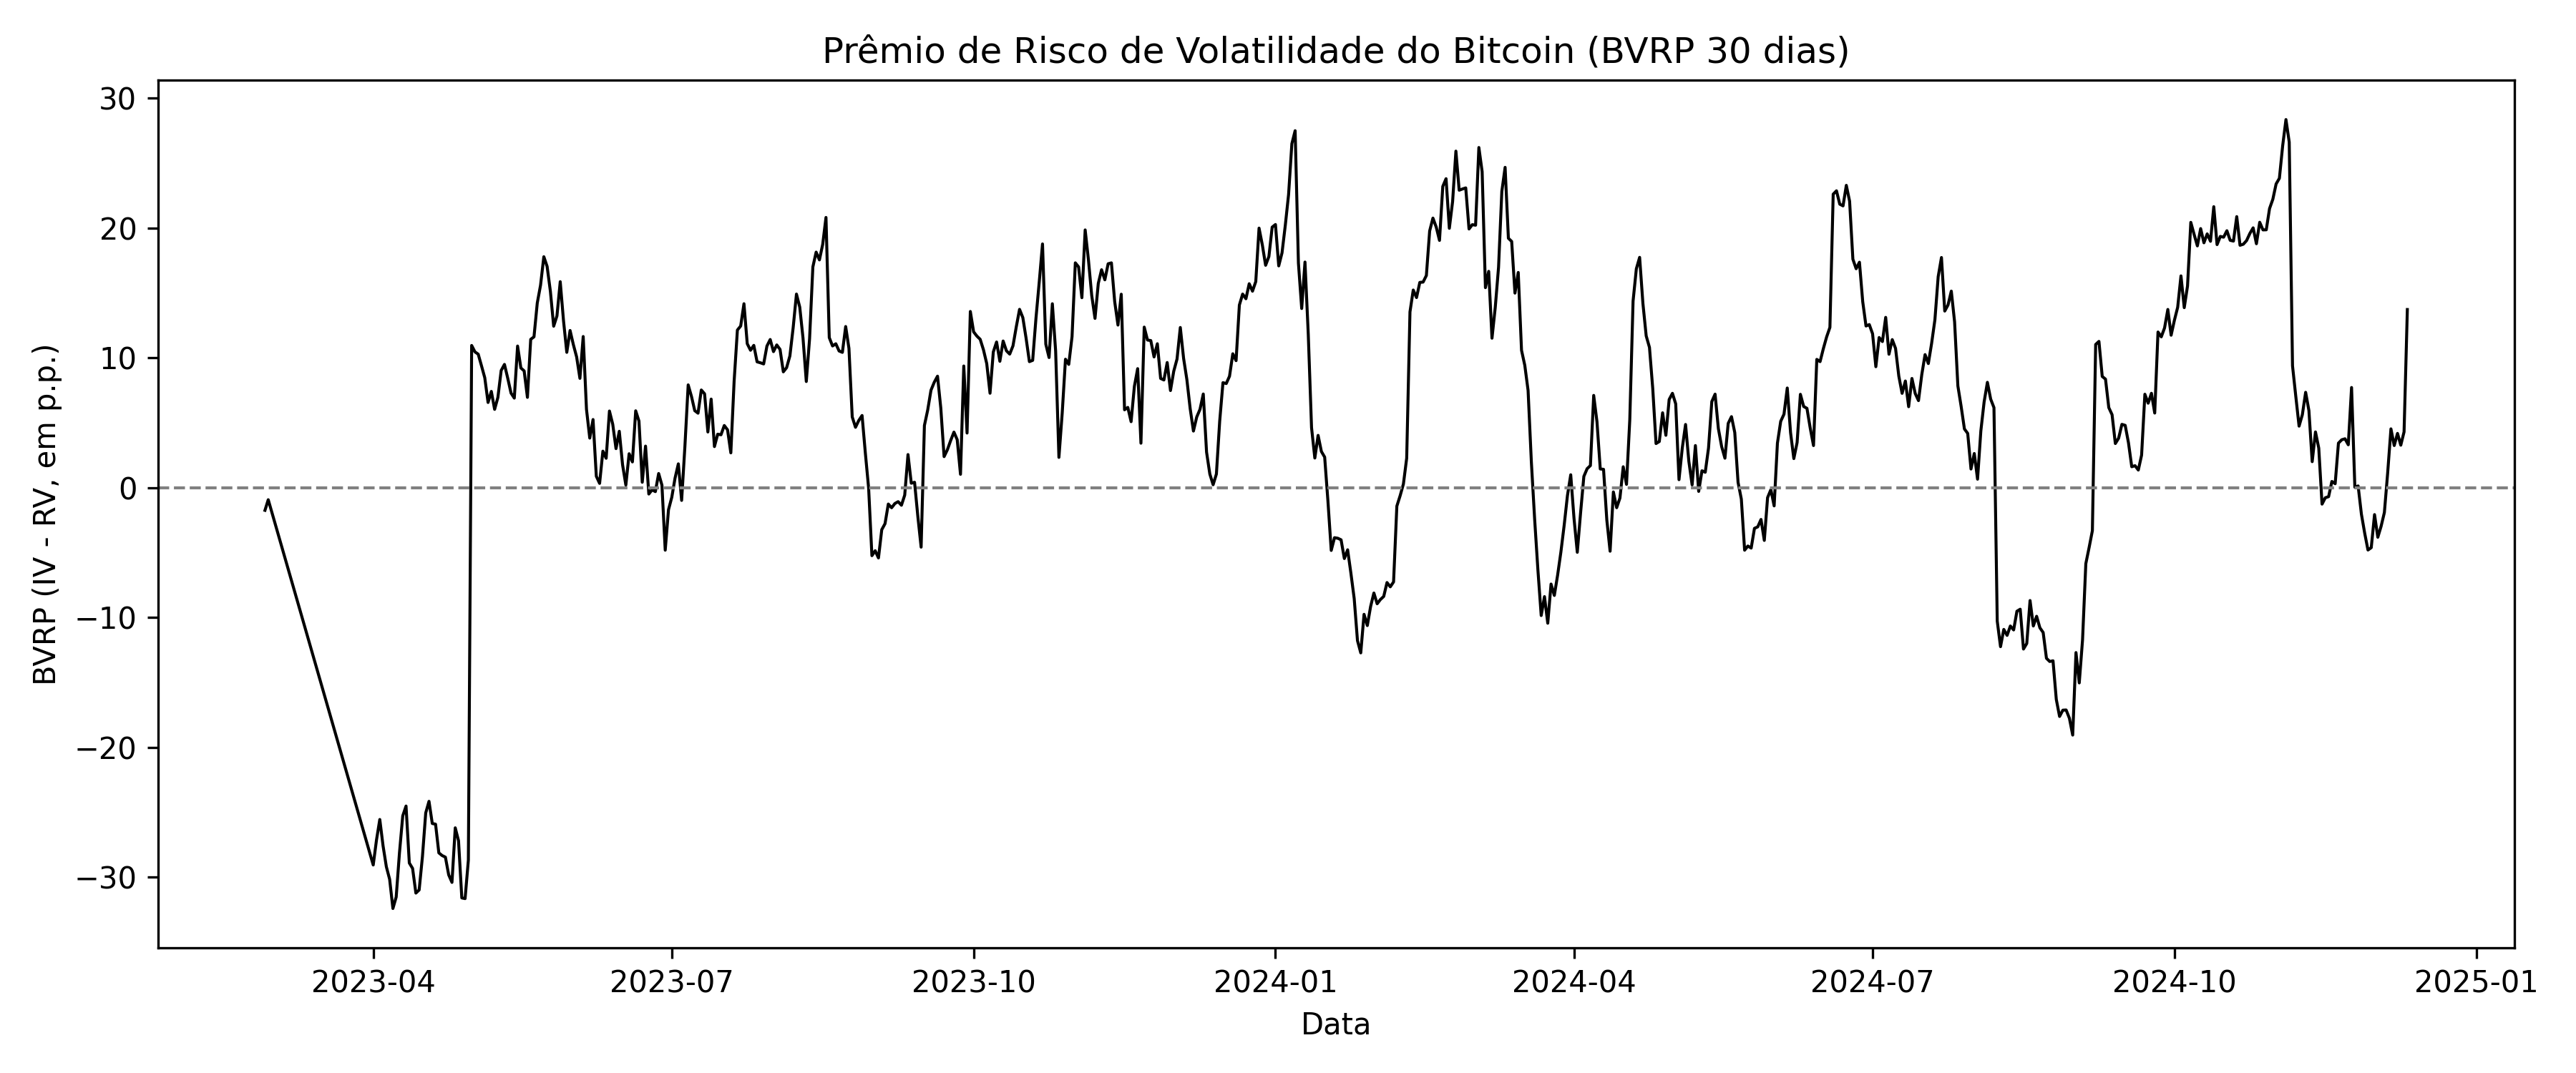
\includegraphics[width=0.92\linewidth]{figs/cap6/fig_6_01_bvrp_timeseries.png}
\caption{Prêmio de risco de volatilidade do Bitcoin (BVRP 30 dias) --- série temporal.}
\label{fig:cap6_bvrp_ts}
\end{figure}
}{}

% =========================================================
\section{Definição do alvo preditivo e desenho experimental}
\label{sec:cap6_target_definition}
% =========================================================

O foco empírico recai sobre a previsão do BVRP em horizonte curto, de forma
estritamente fora da amostra. A lógica é reproduzir um ambiente de decisão
realista: as variáveis explicativas observadas no instante $t$ são utilizadas
para produzir previsões sobre o nível do BVRP em $t+1$.

\subsection{Alvo preditivo: horizonte de 1 dia à frente}
\label{subsec:cap6_target_1d}

Define-se como variável-alvo o valor observado um dia à frente:
\begin{equation}
\text{BVRP}_{t+1} = \text{shift}\!\left(\text{BVRP}_{t},\,-1\right).
\label{eq:cap6_target}
\end{equation}
Assim, todas as variáveis explicativas são observadas em $t$, enquanto o alvo
corresponde ao prêmio de risco em $t+1$.

Essa escolha é motivada por três razões. Primeiro, reflete um ambiente de previsão
economicamente relevante, no qual decisões no presente dependem de expectativas
futuras. Segundo, evita viés de antecipação (\textit{look-ahead bias}), pois
nenhuma informação futura é utilizada na estimação. Terceiro, estabelece um desafio
empírico claro: como o BVRP exibe alta persistência em frequência diária, modelos
devem superar \textit{benchmarks} temporais fortes para demonstrar ganho incremental
genuíno.

\subsection{Divisão temporal: treino, validação e teste}
\label{subsec:cap6_time_split}

A avaliação segue um desenho experimental estritamente fora da amostra, com
divisão temporal da base em três subconjuntos disjuntos: \textit{treinamento},
\textit{validação} e \textit{teste}. A divisão respeita a ordem cronológica, sem
embaralhamento, preservando a estrutura temporal da série.

Os intervalos do experimento são sumarizados na Tabela~\ref{tab:cap6_split_summary}.

\begin{table}[H]
\centering
\caption{Resumo da divisão temporal (alvo: $\text{BVRP}_{t+1}$)}
\label{tab:cap6_split_summary}
\footnotesize
\begin{tabular}{lrrll}
\toprule
Conjunto & Observações & Proporção & Data inicial & Data final \\
\midrule
Treino    & 435 & 70\% & 2023-02-27 & 2024-06-06 \\
Validação &  93 & 15\% & 2024-06-07 & 2024-09-07 \\
Teste     &  94 & 15\% & 2024-09-08 & 2024-12-10 \\
\bottomrule
\end{tabular}
\end{table}

O conjunto de treinamento é utilizado para estimação dos parâmetros dos modelos.
O conjunto de validação é utilizado para seleção de hiperparâmetros e comparação
preliminar entre especificações. O conjunto de teste é reservado para avaliação
final fora da amostra, não sendo utilizado em nenhuma etapa de ajuste ou escolha
de modelos, garantindo assim a integridade do protocolo de avaliação.

% =========================================================
\section{Engenharia de variáveis e controle de vazamento de informação}
\label{sec:cap6_features}
% =========================================================

Esta seção descreve a construção da matriz de variáveis explicativas e os
procedimentos adotados para evitar vazamento de informação (\textit{data leakage}).
Todas as decisões são guiadas pelo princípio de que apenas informações disponíveis
no tempo $t$ podem ser utilizadas para prever $\text{BVRP}_{t+1}$.

\subsection{Seleção de variáveis explicativas}
\label{subsec:cap6_features_selection}

A matriz de preditores é composta por variáveis diretamente relacionadas à dinâmica
do mercado de Bitcoin e à formação do prêmio de risco de volatilidade:
\begin{itemize}
    \item \textbf{close}: preço de fechamento do Bitcoin no mercado à vista;
    \item \textbf{ret}: retorno logarítmico diário do ativo;
    \item \textbf{rv\_30d}: volatilidade realizada em janela móvel de 30 dias;
    \item \textbf{iv\_30d}: volatilidade implícita associada a opções com maturidade de 30 dias.
\end{itemize}

Variáveis que incorporam explicitamente informação futura são excluídas. Em
particular, séries com prefixo \texttt{ret\_fut\_} não são utilizadas como entradas
dos modelos, e o próprio BVRP é incluído apenas na forma defasada em um período.

\subsection{Padronização das variáveis explicativas}
\label{subsec:cap6_scaling}

Como as variáveis explicativas apresentam escalas distintas, aplica-se padronização
do tipo \textit{z-score} antes da estimação:
\begin{equation}
x^{\ast}_{j,t} = \frac{x_{j,t} - \mu_j}{\sigma_j},
\end{equation}
em que $\mu_j$ e $\sigma_j$ são calculados exclusivamente com base no conjunto de
treinamento. Os parâmetros estimados no treino são então aplicados aos conjuntos de
validação e teste, sem reestimação, evitando vazamento de informação.

\begin{table}[H]
\centering
\caption{Parâmetros de padronização das variáveis explicativas (treino)}
\label{tab:cap6_scaler_stats}
\footnotesize
\begin{tabular}{lrr}
\toprule
Variável & Média (treino) & Desvio-padrão (treino) \\
\midrule
close   & 41.009{,}48 & 15.551{,}59 \\
ret     & 0{,}00248   & 0{,}02597   \\
rv\_30d & 47{,}49     & 16{,}05     \\
iv\_30d & 52{,}27     & 11{,}17     \\
\bottomrule
\end{tabular}
\end{table}

% =========================================================
\section{Modelos \textit{baseline} e \textit{benchmarks} preditivos}
\label{sec:cap6_baselines}
% =========================================================

Antes da estimação de modelos de aprendizado de máquina, são estabelecidos
\textit{benchmarks} de desempenho preditivo. Esses modelos servem como referências
mínimas e ajudam a distinguir ganhos genuínos de resultados que apenas refletem
persistência temporal.

As métricas de avaliação utilizadas são MAE, RMSE e $R^2$, reportadas
separadamente para validação e teste. Como o alvo é o \textit{nível} do BVRP em
$t+1$, valores elevados de $R^2$ são esperados quando a série exibe forte
persistência em frequência diária; portanto, a interpretação econômica deve
priorizar ganhos relativos frente aos baselines.

\subsection{Baselines temporais}
\label{subsec:cap6_baselines_temporais}

Dois baselines temporais fortes são adotados:
\begin{itemize}
    \item \textbf{Último valor} (\textit{last value}):
    $\widehat{\text{BVRP}}_{t+1} = \text{BVRP}_{t}$;
    \item \textbf{Média móvel} com $k=5$:
    $\widehat{\text{BVRP}}_{t+1} = \tfrac{1}{5}\sum_{j=0}^{4}\text{BVRP}_{t-j}$.
\end{itemize}

A Tabela~\ref{tab:cap6_baselines} apresenta os resultados. Observa-se que o
baseline de último valor é extremamente competitivo, consistente com a persistência
temporal do BVRP em base diária.

\begin{table}[H]
\centering
\caption{Desempenho dos baselines temporais}
\label{tab:cap6_baselines}
\footnotesize
\begin{tabular}{llrrr}
\toprule
Modelo & Conjunto & MAE & RMSE & $R^2$ \\
\midrule
baseline\_last\_value & Val  & 2{,}022 & 3{,}265 & 0{,}922 \\
baseline\_ma\_5       & Val  & 3{,}699 & 5{,}198 & 0{,}803 \\
baseline\_last\_value & Test & 1{,}759 & 2{,}861 & 0{,}893 \\
baseline\_ma\_5       & Test & 2{,}861 & 4{,}227 & 0{,}767 \\
\bottomrule
\end{tabular}
\end{table}

% =========================================================
\section{Modelos lineares regulares}
\label{sec:cap6_linear}
% =========================================================

Após o estabelecimento de \textit{benchmarks} preditivos, esta seção avalia modelos
lineares regulares. O objetivo é investigar se relações lineares entre o BVRP futuro
e variáveis observadas em $t$ produzem ganho incremental fora da amostra.

Consideram-se três modelos: MQO, Ridge ($L_2$) e Lasso ($L_1$). O parâmetro de
regularização é selecionado por desempenho no conjunto de validação.

\subsection{Resultados e interpretação}
\label{subsec:cap6_linear_results}

A Tabela~\ref{tab:cap6_linear_metrics} reporta o desempenho. Os três modelos
exibem resultados praticamente indistinguíveis, sugerindo baixa sensibilidade à
regularização no problema analisado e reforçando o papel da persistência do BVRP
como \textit{benchmark} dominante em horizonte de 1 dia.

\begin{table}[H]
\centering
\caption{Desempenho dos modelos lineares}
\label{tab:cap6_linear_metrics}
\footnotesize
\begin{tabular}{llrrr}
\toprule
Modelo & Conjunto & MAE & RMSE & $R^2$ \\
\midrule
ols   & Val  & 2{,}187 & 3{,}273 & 0{,}922 \\
ridge & Val  & 2{,}187 & 3{,}273 & 0{,}922 \\
lasso & Val  & 2{,}187 & 3{,}273 & 0{,}922 \\
ols   & Test & 1{,}887 & 2{,}867 & 0{,}893 \\
ridge & Test & 1{,}887 & 2{,}867 & 0{,}893 \\
lasso & Test & 1{,}887 & 2{,}867 & 0{,}893 \\
\bottomrule
\end{tabular}
\end{table}

Em termos econômicos, os sinais estimados são consistentes com a definição do
prêmio de risco de volatilidade: a volatilidade implícita contribui positivamente
e a volatilidade realizada negativamente para o prêmio de risco. A
Figura~\ref{fig:cap6_linear_coef} ilustra os coeficientes estimados sobre
\textit{features} padronizadas.

\IfFileExists{figs/cap6/fig_6_09_linear_coefficients.png}{
\begin{figure}[H]
\centering
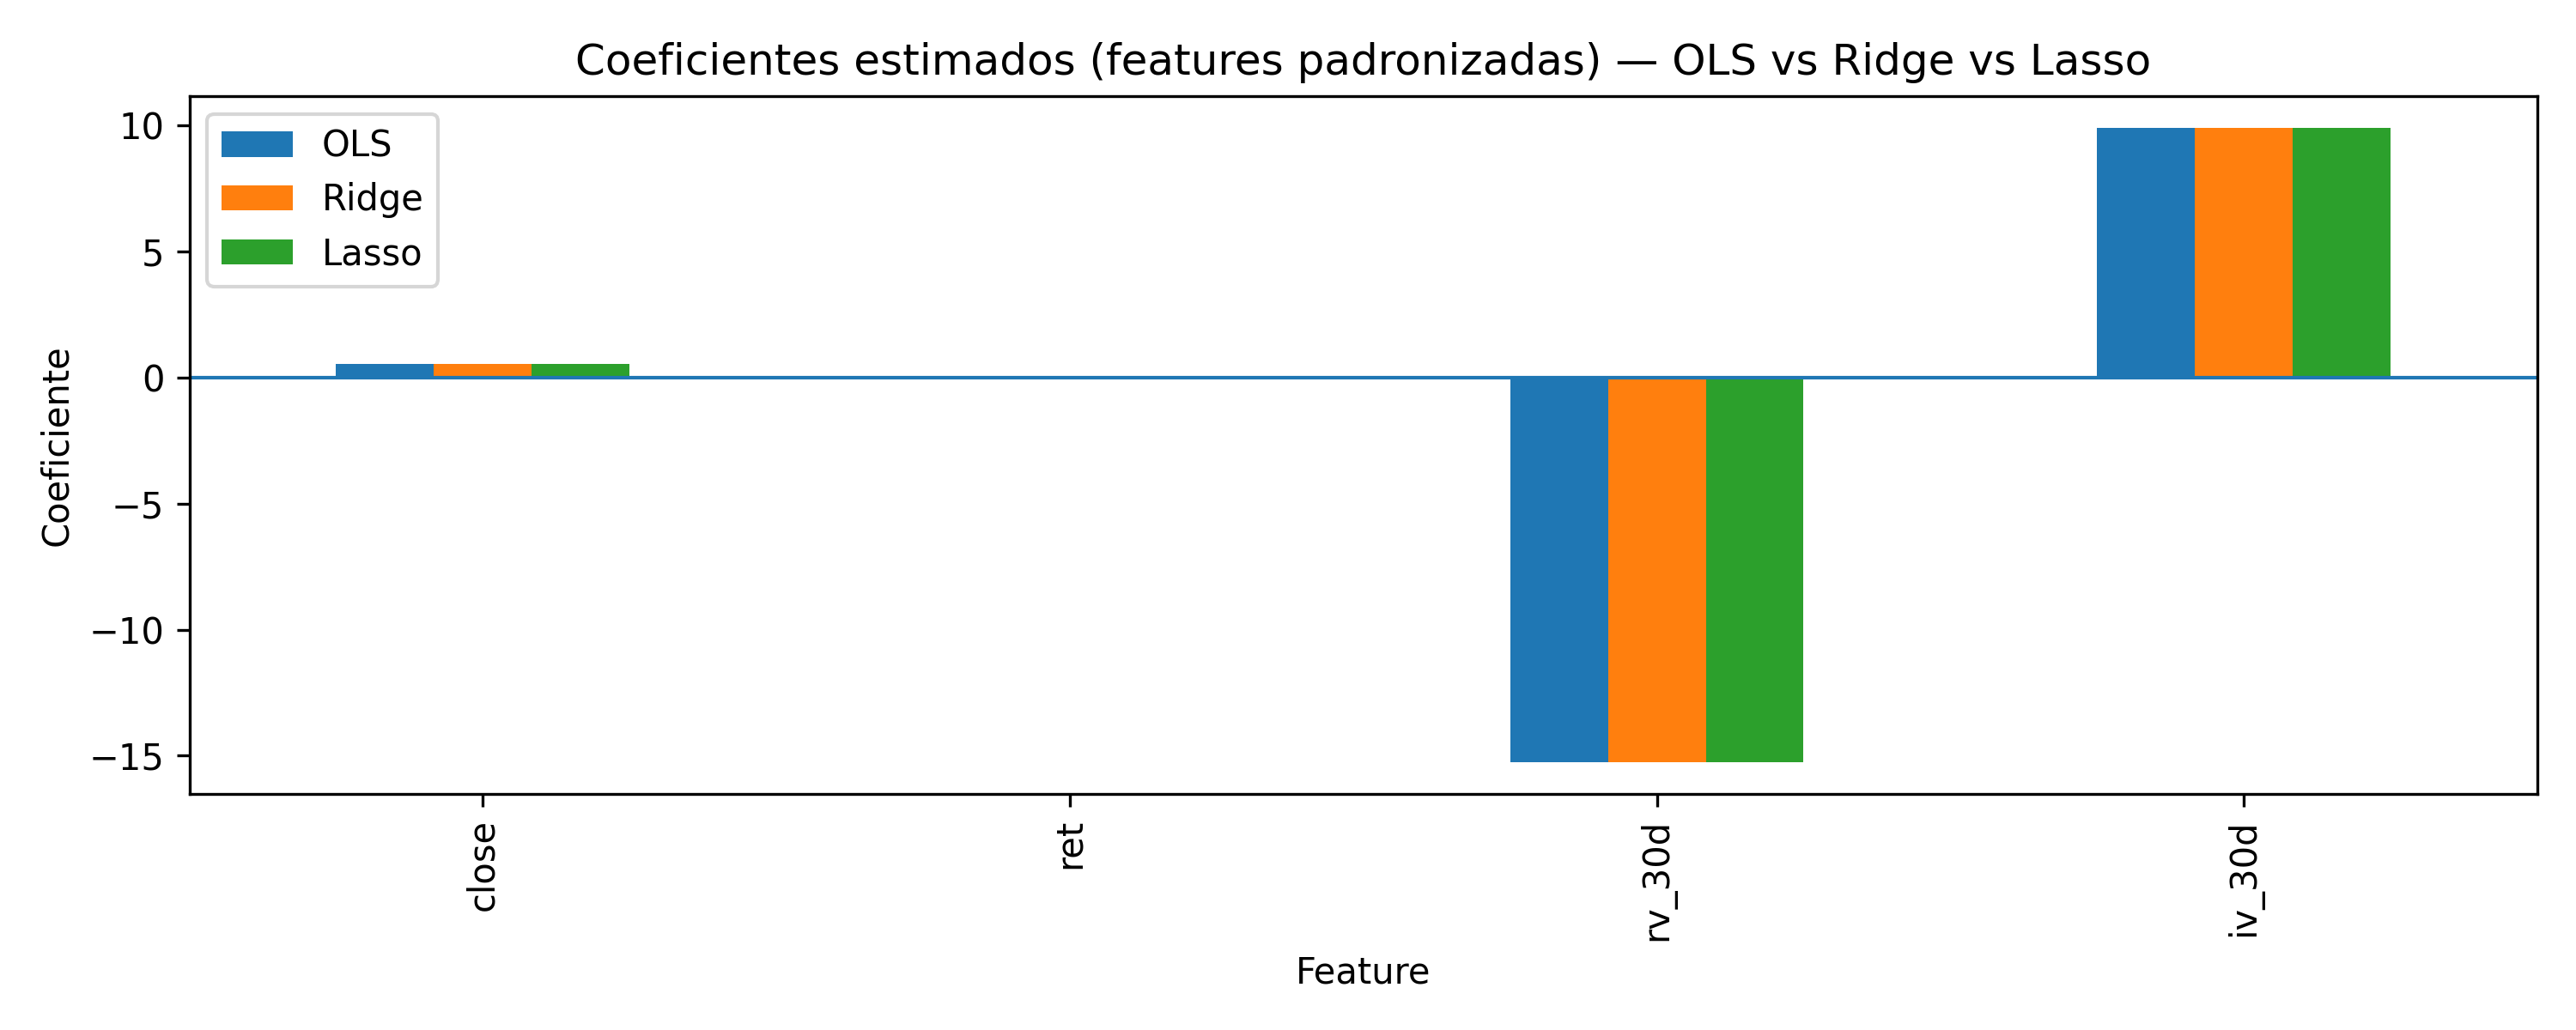
\includegraphics[width=0.88\linewidth]{figs/cap6/fig_6_09_linear_coefficients.png}
\caption{Coeficientes estimados (\textit{features} padronizadas): MQO vs Ridge vs Lasso.}
\label{fig:cap6_linear_coef}
\end{figure}
}{}

% =========================================================
\section{Modelos baseados em árvores}
\label{sec:cap6_trees}
% =========================================================

Esta seção investiga modelos baseados em árvores de decisão, capazes de capturar
não linearidades e interações sem impor forma funcional paramétrica. Foram avaliados
uma árvore de decisão e uma floresta aleatória, com seleção de hiperparâmetros
baseada no conjunto de validação.

\subsection{Resultados e importância de variáveis}
\label{subsec:cap6_trees_results}

A Tabela~\ref{tab:cap6_trees_metrics} apresenta o desempenho. Em geral, os modelos
baseados em árvores não superam os modelos lineares nem o baseline de persistência,
sugerindo que a informação adicional capturada por não linearidades e interações é
limitada no contexto analisado, ou que a amostra disponível é insuficiente para
sustentar ganhos robustos fora da amostra.

\begin{table}[H]
\centering
\caption{Desempenho dos modelos baseados em árvores}
\label{tab:cap6_trees_metrics}
\footnotesize
\begin{tabular}{llrrr}
\toprule
Modelo & Conjunto & MAE & RMSE & $R^2$ \\
\midrule
decision\_tree\_tuned & Val  & 5{,}564 & 6{,}747 & 0{,}668 \\
decision\_tree\_tuned & Test & 3{,}404 & 4{,}498 & 0{,}736 \\
random\_forest\_tuned & Val  & 6{,}372 & 7{,}843 & 0{,}551 \\
random\_forest\_tuned & Test & 2{,}750 & 3{,}749 & 0{,}817 \\
\bottomrule
\end{tabular}
\end{table}

A Figura~\ref{fig:cap6_rf_importance} reporta a importância das variáveis no modelo
de floresta aleatória, evidenciando papel dominante das medidas de volatilidade
realizada e implícita na previsão do BVRP.

\IfFileExists{figs/cap6/fig_6_10_rf_feature_importance.png}{
\begin{figure}[H]
\centering
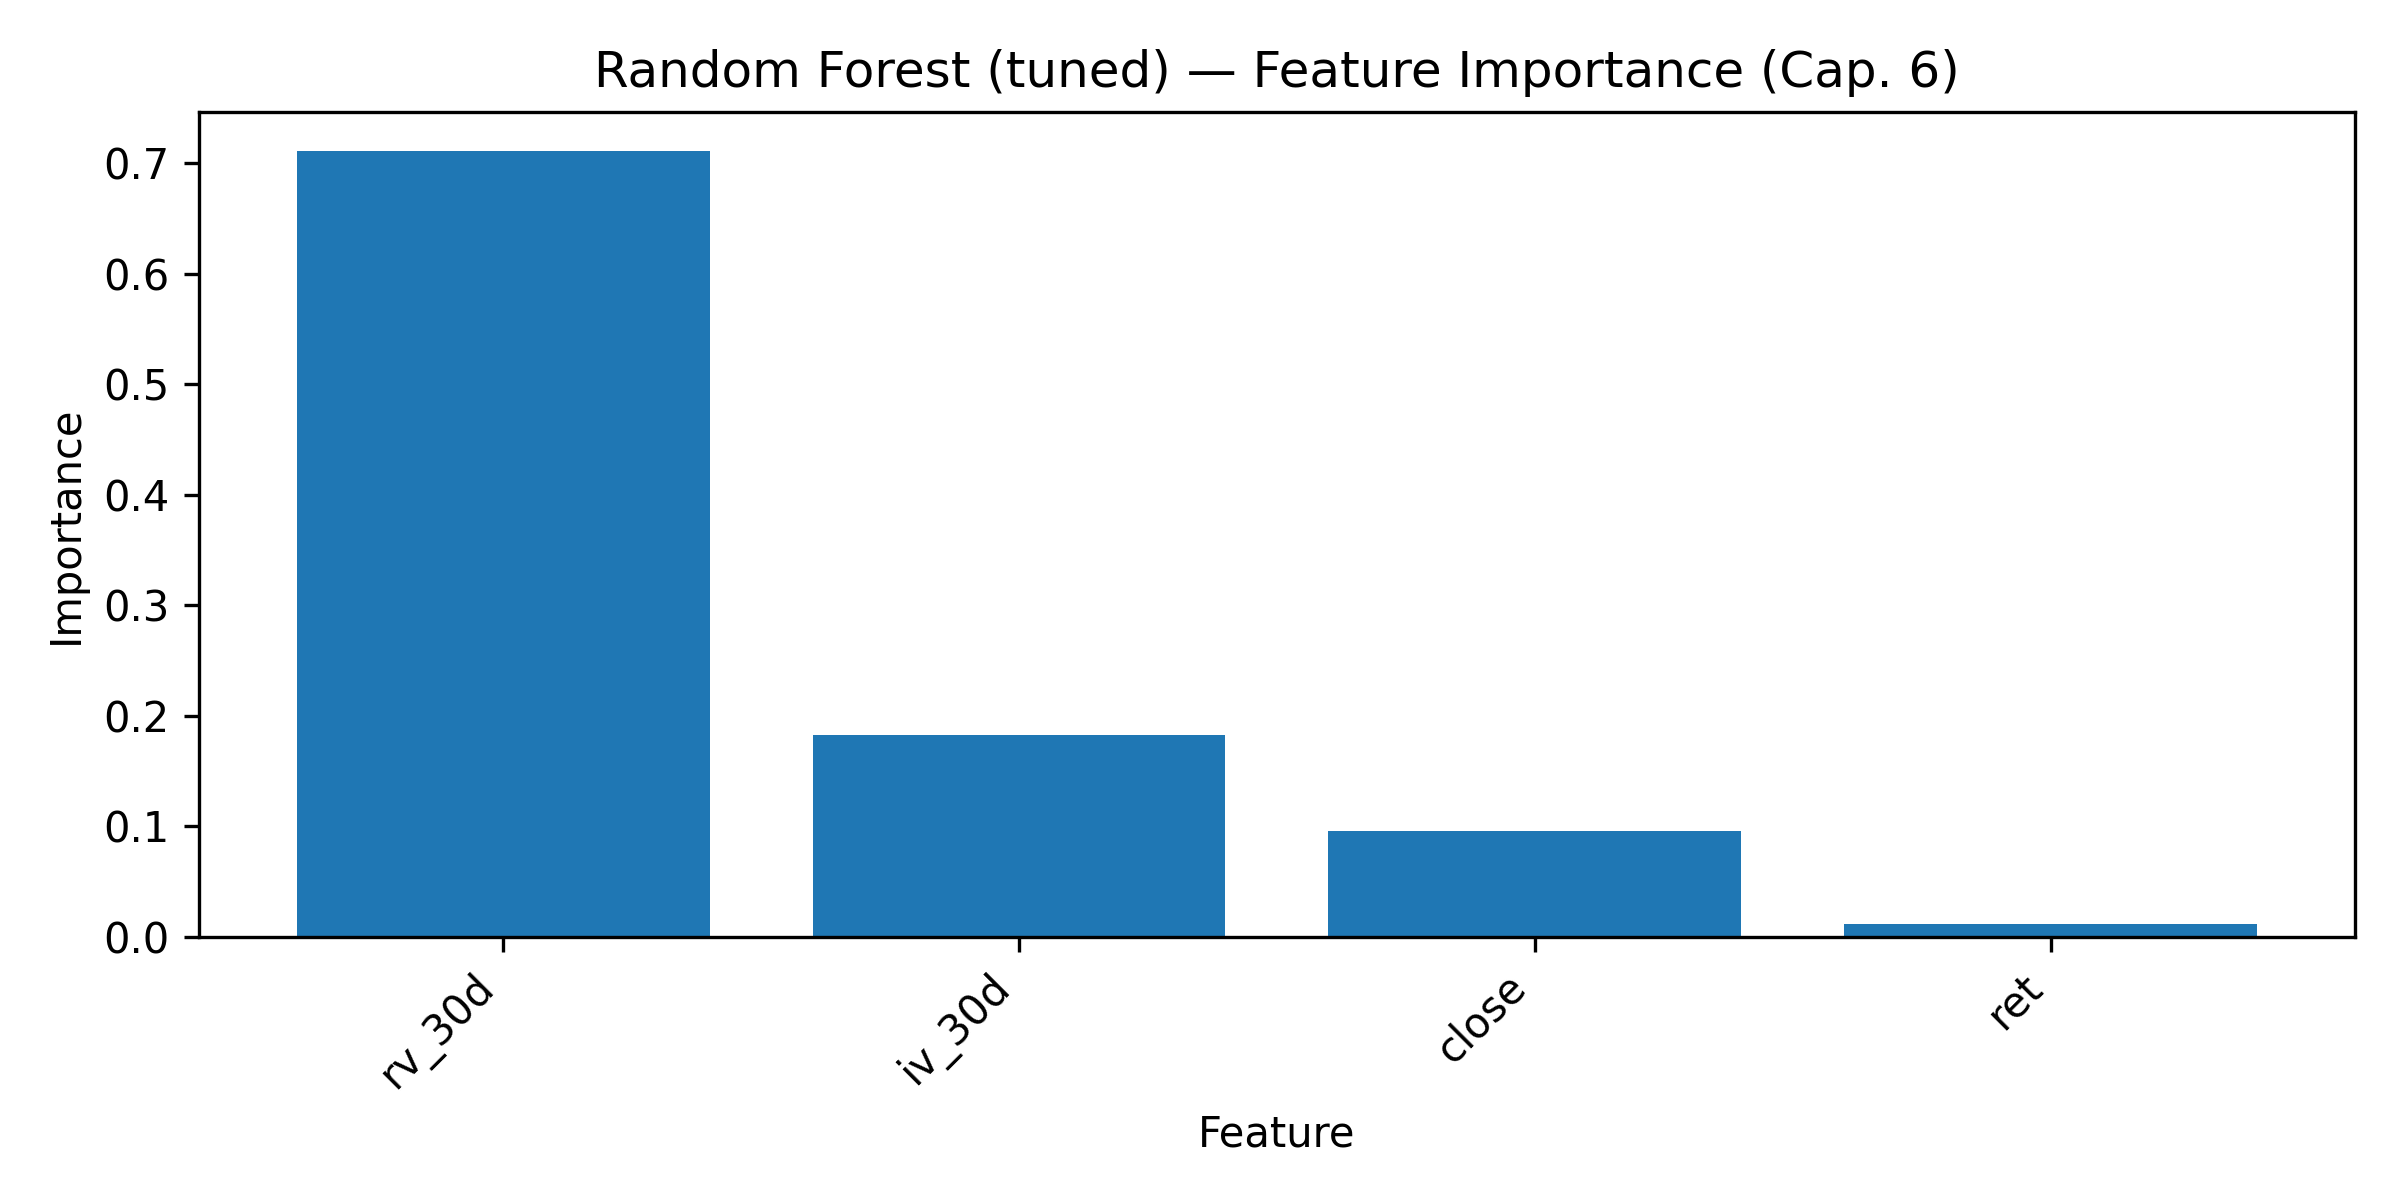
\includegraphics[width=0.88\linewidth]{figs/cap6/fig_6_10_rf_feature_importance.png}
\caption{Importância de variáveis na floresta aleatória (ajustado).}
\label{fig:cap6_rf_importance}
\end{figure}
}{}

% =========================================================
\section{Modelos não lineares avançados: métodos de \textit{boosting}}
\label{sec:cap6_boosting}
% =========================================================

Esta seção avalia modelos não lineares avançados baseados em \textit{boosting}, que
combinam sequencialmente árvores rasas para reduzir vieses e capturar padrões
residuais. Foram comparados: (i)~\textit{Gradient Boosting Regression Trees}
(GBRT), (ii)~XGBoost e (iii)~LightGBM. A seleção de hiperparâmetros é guiada pelo
conjunto de validação.

\subsection{Resultados}
\label{subsec:cap6_boosting_results}

A Tabela~\ref{tab:cap6_boosting_metrics} apresenta o desempenho. Entre os métodos
de \textit{boosting}, o XGBoost apresenta o melhor resultado fora da amostra na
configuração considerada, embora não supere o baseline de persistência nem os
modelos lineares no período analisado.

\begin{table}[H]
\centering
\caption{Desempenho dos modelos de \textit{boosting}}
\label{tab:cap6_boosting_metrics}
\footnotesize
\begin{tabular}{llrrr}
\toprule
Modelo & Conjunto & MAE & RMSE & $R^2$ \\
\midrule
gbrt     & Val  & 5{,}215 & 6{,}351 & 0{,}706 \\
xgboost  & Val  & 5{,}173 & 6{,}323 & 0{,}708 \\
lightgbm & Val  & 5{,}352 & 6{,}616 & 0{,}681 \\
gbrt     & Test & 2{,}436 & 3{,}369 & 0{,}852 \\
xgboost  & Test & 2{,}457 & 3{,}348 & 0{,}854 \\
lightgbm & Test & 3{,}121 & 4{,}014 & 0{,}790 \\
\bottomrule
\end{tabular}
\end{table}

Para fins de comparação, as Figuras~\ref{fig:cap6_rf_real_vs_pred}
e~\ref{fig:cap6_xgb_real_vs_pred} apresentam os gráficos de dispersão entre
$\text{BVRP}_{t+1}$ real e previsto no conjunto de teste para a floresta aleatória
(melhor modelo baseado em árvores) e o XGBoost (melhor método de
\textit{boosting}), respectivamente. A aderência à linha diagonal é visível nos
dois casos, reflexo da alta persistência da série, porém com dispersão maior do
que a observada no baseline de último valor.

\IfFileExists{figs/cap6/fig_6_11_rf_real_vs_pred.png}{
\begin{figure}[H]
\centering
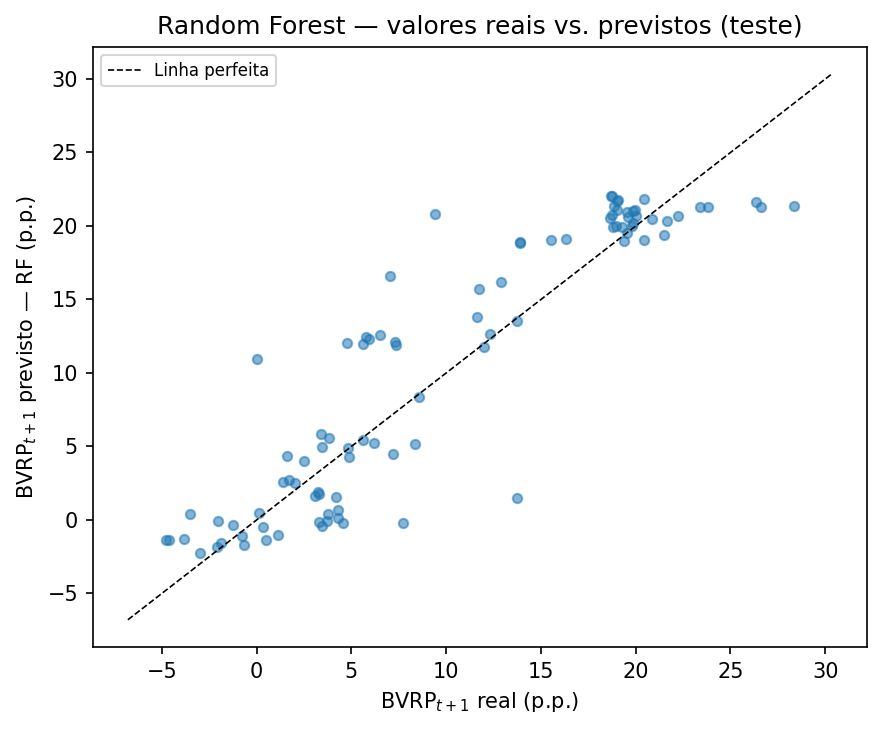
\includegraphics[width=0.78\linewidth]{figs/cap6/fig_6_11_rf_real_vs_pred.png}
\caption{floresta aleatória --- $\text{BVRP}_{t+1}$ real vs.\ previsto no conjunto de teste (p.p.).}
\label{fig:cap6_rf_real_vs_pred}
\end{figure}
}{}

\IfFileExists{figs/cap6/fig_6_12_xgb_real_vs_pred.png}{
\begin{figure}[H]
\centering
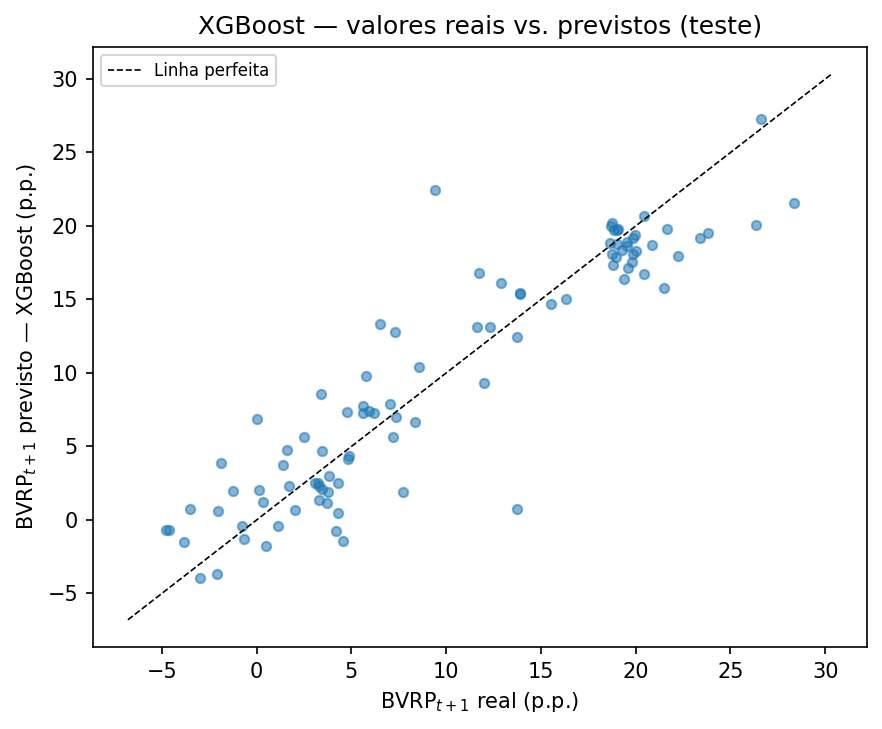
\includegraphics[width=0.78\linewidth]{figs/cap6/fig_6_12_xgb_real_vs_pred.png}
\caption{XGBoost --- $\text{BVRP}_{t+1}$ real vs.\ previsto no conjunto de teste (p.p.).}
\label{fig:cap6_xgb_real_vs_pred}
\end{figure}
}{}

\FloatBarrier

% =========================================================
\section{Evidência complementar e conexão com os resultados econométricos}
\label{sec:cap6_multihorizon_ols}
% =========================================================

Como evidência complementar, reporta-se a análise econométrica multihorizonte
apresentada no Capítulo~\ref{chap:resultados_ols}, na qual se avalia a relação
entre o BVRP observado em $t$ e retornos futuros do Bitcoin em diferentes
horizontes. Essa evidência não constitui o alvo principal deste capítulo (previsão
do BVRP em $t+1$), mas ajuda a contextualizar a relevância econômica do prêmio de
risco e a motivar o interesse por modelos preditivos.

A Tabela~\ref{tab:ols_basico_multihoriz},
apresentada no Capítulo~\ref{chap:resultados_ols},
reporta os resultados do modelo básico de regressão de retornos futuros sobre
o nível corrente do BVRP em seis horizontes. Conforme demonstrado naquele
capítulo, o BVRP não apresenta capacidade preditiva linear estatisticamente
significativa em nenhum dos horizontes analisados, com o menor valor-$p$
observado sendo de $0{,}241$ ($h=1$). A ausência de previsibilidade linear ---
robusta à reamostragem em blocos e à correção para múltiplos testes ---
motiva diretamente o uso de modelos não paramétricos aplicados neste capítulo,
capazes de capturar relações não lineares e interações entre preditores que
regressões lineares simples não detectam.

De forma geral, a evidência é consistente com a interpretação de que o prêmio de
risco carrega informação econômica relevante para a previsão de retornos, mas que
a extração de ganhos preditivos incrementais sobre o \textit{nível} do BVRP é
desafiadora quando se impõe um protocolo estritamente fora da amostra e se compara
contra \textit{benchmarks} fortes de persistência temporal.

% =========================================================
\section{Comparação global e \textit{ranking} final}
\label{sec:cap6_ranking}
% =========================================================

Nesta seção, consolida-se o desempenho preditivo de todas as famílias de modelos
avaliadas. O critério principal de ordenação é o RMSE no conjunto de teste, por
penalizar erros extremos de forma mais severa.

A Tabela~\ref{tab:cap6_ranking_test} apresenta o \textit{ranking} final, ordenado
por RMSE crescente. Observa-se que o baseline de persistência permanece como o
melhor preditor, seguido de perto pelos modelos lineares. Entre os modelos não
lineares, o XGBoost se destaca, porém com desempenho inferior às abordagens mais
simples no período analisado.

\begin{table}[H]
\centering
\caption{\textit{Ranking} final no conjunto de teste (ordenado por RMSE)}
\label{tab:cap6_ranking_test}
\footnotesize
\begin{tabular}{rllrrr}
\toprule
Rank & Modelo & Família & MAE & RMSE & $R^2$ \\
\midrule
 1 & baseline\_last\_value  & baselines & 1{,}759 & 2{,}861 & 0{,}893 \\
 2 & ols                    & linear    & 1{,}887 & 2{,}867 & 0{,}893 \\
 3 & ridge                  & linear    & 1{,}887 & 2{,}867 & 0{,}893 \\
 4 & lasso                  & linear    & 1{,}887 & 2{,}867 & 0{,}893 \\
 5 & xgboost                & boosting  & 2{,}457 & 3{,}348 & 0{,}854 \\
 6 & gbrt                   & boosting  & 2{,}436 & 3{,}369 & 0{,}852 \\
 7 & random\_forest\_tuned  & trees     & 2{,}750 & 3{,}749 & 0{,}817 \\
 8 & lightgbm               & boosting  & 3{,}121 & 4{,}014 & 0{,}790 \\
 9 & baseline\_ma\_5        & baselines & 2{,}861 & 4{,}227 & 0{,}767 \\
10 & decision\_tree\_tuned  & trees     & 3{,}404 & 4{,}498 & 0{,}736 \\
\bottomrule
\end{tabular}
\end{table}

% =========================================================
\section{Discussão econômica dos resultados}
\label{sec:cap6_discussion}
% =========================================================

Os resultados empíricos indicam que a maior parte da capacidade preditiva fora da
amostra decorre da persistência temporal do BVRP em frequência diária, o que
estabelece um \textit{benchmark} forte e difícil de ser superado. Esse padrão sugere
elevado grau de inércia na dinâmica do prêmio de risco, consistente com ajuste
gradual de expectativas e com fricções de liquidez e de \textit{inventory} no
mercado de derivativos.

Os modelos lineares exibem desempenho muito próximo ao baseline, sugerindo que
variáveis contemporâneas de preço, retornos e volatilidades adicionam informação
incremental limitada além da persistência. Ainda assim, a interpretação dos
coeficientes é economicamente plausível: a volatilidade implícita contribui
positivamente e a volatilidade realizada negativamente para o prêmio de risco, em
linha com a definição do BVRP como diferencial entre expectativas (IV) e
realizações (RV).

Modelos não lineares avançados (\textit{boosting}) apresentam ganhos marginais em
relação a árvores individuais, mas não superam de forma robusta as abordagens mais
simples fora da amostra. Esse resultado é compatível com a literatura: quando o
conteúdo informacional adicional é limitado e a amostra é relativamente curta,
modelos flexíveis tendem a capturar ruído específico do período analisado, reduzindo
a capacidade de generalização.

Do ponto de vista aplicado, a evidência sugere que estratégias dependentes de
previsão diária do nível do BVRP devem priorizar modelos parcimoniosos e
\textit{benchmarks} fortes, uma vez que complexidade adicional pode elevar o risco
de sobreajuste e o custo de implementação sem ganhos econômicos proporcionais.

% =========================================================
\section{Conclusão do capítulo}
\label{sec:cap6_conclusion}
% =========================================================

Este capítulo investigou a previsibilidade fora da amostra do prêmio de risco de
volatilidade do Bitcoin por meio de uma gama de modelos estatísticos e de
aprendizado de máquina, incluindo baselines temporais, modelos lineares
regulares, modelos baseados em árvores e métodos de \textit{boosting}.

O desenho empírico foi intencionalmente rigoroso, com divisão temporal, definição
explícita de horizonte de previsão e controle de \textit{look-ahead bias}. Os
resultados mostram que a persistência temporal do BVRP estabelece um
\textit{benchmark} particularmente forte, difícil de ser superado. Modelos lineares
capturam relações economicamente plausíveis com medidas de volatilidade, mas não
produzem ganhos robustos além do baseline. Modelos não lineares avançados exibem
desempenho inferior às abordagens mais simples na amostra analisada, sugerindo
limites práticos à previsibilidade incremental do nível do BVRP em frequência
diária no período considerado.

No próximo capítulo, os resultados são integrados e interpretados à luz das
implicações para modelagem preditiva, estratégias condicionais e gestão de risco
no mercado de derivativos de Bitcoin.
